\subsection{Les newsgroups}
\label{newsgroups}
\subsubsection{Pr\'esentation}
Le BR fournit aux \'el\`eves un service de newsgroups, souvent surnomm\'e ``les br''.
Ils fonctionnent un peu comme un forum : chacun peut poster une annonce, poser une question,
 r\'epondre \`a un sujet post\'e par un autre \'el\`eve\ldots\
Ils sont tr\`es utiles pour faire de la pub pour une activit\'e organis\'ee par un binet,
poser une question en cas de probl\`eme, ou tout simplement savoir ce qu'il se passe sur le plat\^al.
Pour qu'ils puissent remplir pleinement ce r\^ole, le BR a \'edict� un certain nombre de r\`egles
que les newsmestres sont charg\'es de faire respecter.

\subsubsection{Les r\`egles}
\begin{itemize}
 \item Pas d'insultes, attaques personnelles, calomnies et autres.
 \item Ne pas dissimuler son identit\'e, et donc utiliser une adresse mail valide
       et un pseudo qui permet de t'identifier par l'interm\'ediaire du TOL.
 \item Pour que les {\it br} restent lisibles, faire des crossposts propres (cf infoBR p11).
 \item Dans le m\^eme ordre d'id\'ee, poster sur le forum adapt\'e:
       les petites annonces vont sur le \ngname{br.pa} et nulle part ailleurs,
       seules les questions concernant directement le BR ont leur place sur le \ngname{br.binet.br}
       (pour les questions d'informatique il y a les \ngname{br.informatique.*}).
 \item Eviter de troller\footnote{poster des messages provocateurs et non constructifs dans le seul but
       de g�n�rer des pol�miques\ldots ou tout simplement entrer dans le jeu de celui qui te provoque
       et poster une centaine de messages inutiles en quelques dizaines de minutes ;)} abusivement
       (sauf sur \ngname{br.binet.polemix} qui sert \`a \c{c}a ;))
 \item Garder son calme (ou \'eviter de poster), mieux vaut une explication dans la vraie vie
       que par {\it br} interpos\'e.
\end{itemize}

\subsubsection{Les diff\'erents newsgroups de frankiz}
Frankiz h\'eberge un grand nombre de newsgroups (plus de 200...),
mais il est probable qu'ils ne t'int\'eressent pas tous.
Pour faire un choix au d\'ebut, en voici une liste non exhaustive
(tu peux aussi t'amuser \`a tous les lire si tu veux devenir newsmestre ;)) :
\begin{itemize}
 \item[\ngname{br.eleves} :] posts g\'en\'eraux int\'eressant potentiellement un grand nombre d'\'el\`eves
 \item[\ngname{br.promo.*} :] pour les posts ne concernant \`a priori qu'une seule promo (Rouje, Jone ou Oranje)
 \item[\ngname{br.kes} :] le newsgroup de la K\`es. Suite \`a un pourrissage abusif de ce br, des restrictions
                 ont \'et\'e mises en place: tout le monde peut lancer une nouvelle discussion sur ce newsgroup,
                 mais seuls les kessiers peuvent r\'epondre.
                 Il sert donc essentiellement \`a la K\`es pour faire une annonce, ou aux \'el\`eves
                 pour poser une question aux kessiers (note: il n'est pas non plus interdit
                 de se d\'eplacer \`a la K\`es pour poser ta question directement)
 \item[\ngname{br.binet.ton\_binet} :] chaque binet a son newsgroup. Il sert le plus souvent pour la communication interne
                              du binet, ses annonces ou \`a poser une question au dit binet.
                              Dans le cas d'un nouveau binet, le BR peut lui cr\'eer un newsgroup, mais uniquement
                              apr\`es que le binet ait \'et\'e cr\'e\'e dans les r\`egles \`a la K\`es.
 \item[\ngname{br.binet.br} :] comme son nom l'indique, il s'agit du newsgroup du binet r\'eseau.
                      \`A utiliser pour les questions ayant un lien \emph{direct} avec le BR.
                      Pour les autres questions li\'ees \`a l'informatique,
                      il convient d'utiliser les newsgroups suivants:
 \item[\ngname{br.informatique.reseau} :] pour tout ce qui a trait au r\'eseau
 \item[\ngname{br.informatique.windows/linux/mac} :] selon ton OS
 \item[\ngname{br.informatique.divers} :] pour le reste
 \item[\ngname{br.binet.lose} et \ngname{br.binet.suba\"isse} :] pour raconter tes meilleures loses/suba\"isses et d\'ecouvrir
       que tu n'es pas le seul \`a loser. Pour la diff\'erence subtile entre une lose et une suba\"isse,
       contacter le binet suba\"isse (on n'a pas compris).
 \item[\ngname{br.binet.polemix} :] le forum pour troller par excellence.
                           Attention, essayer de suivre les discussions qui y ont trouv\'e refuge
                           peut prendre \'enorm\'ement de temps.
 \item[\ngname{br.communaut\'e.*} :] les newsgroups de diff\'erentes communaut\'es
                            (religieuses, musicales, g\'eographiques ou autres)
 \item[\ngname{br.enseignement} :] pour tout ce qui a trait \`a l'enseignement.
 \item[\ngname{br.section.ta\_section\_sportive} :] le newsgroup de ta section.
                                           Utile pour savoir ce qu'il s'y passe et planifier les activit\'es.
 \item[\ngname{br.pa} :] pour les petites annonces. Merci de les poster ici et pas ailleurs.
 \item[\ngname{br.test} :] quand tu veux tester un truc sur les newsgroups,
                  viens le faire ici plut\^ot que de pourrir un br utile.
 \item[\ngname{br.trash} :] pour les craquages.
 \item[\ngname{public.*} :] les newsgroups \emph{accessibles \`a l'ensemble du personnel de l'\'ecole}.
                   Il y a peu de messages post�s, mais ils peuvent parfois se r�veler utiles.
\end{itemize}

Il arrive parfois que certains newsgroups temporaires soient cr\'e\'es
pour des \'ev\`enements particuliers (campagne K\`es).
Leur cr\'eation sera annonc\'e le plus souvent sur \fkz ou sur le \ngname{br.eleves}.

\subsubsection{Autres newsgroups}
Le site \url{polytechnique.org} dispose de son propre service de newsgroups.
Il sont accessibles \`a tous les polytechniciens, qu'ils soient actuellement sur le campus
ou membres de promos pr\'ec\'edentes.
Pour plus d'informations, consulte \server{www.polytechnique.org}.

Il est aussi possible d'acc\'eder \`a certains newsgroups ext\'erieurs \`a l'\'ecole via \server{polynews}.
Ce serveur de la DSI est synchronis\'e avec l'ext\'erieur.
Si tu cherches un newsgroup qui ne s'y trouve pas, n'h\'esite pas \`a demander aux newsmestres
(cf section suivante).

\subsubsection{Les newsmestres}
Les newsmestres sont les membres du BR charg\'es de l'administration et de la mod\'eration des newsgroups.
Leur but est de maintenir les newsgroups dans un \'etat correct, pour que tout le monde puisse en profiter
et trouver ce qu'il y cherche.
Ne prends donc pas une remarque de leur part comme une attaque personnelle\ldots

Pour les contacter: \mail{news@frankiz.polytechnique.fr}.

\subsection{Poster sur plusieurs newsgroups...}

Il se peut qu'un jour tu veuilles annoncer un grand �v�nement sur les newsgroups,
et que pour ceci tu aies envie de poster ton message sur plusieurs newsgroups.
Alors avant de commencer � poster sur un newsgroup, faire copier-coller,
poster sur le newsgroup suivant, etc., lis ce qui suit et apprend � gagner du temps,
et simplifier ta vie et celle de tes camarades.

\subsubsection{Qu'est-ce qu'un crosspost ?}
Un crosspost permet de poster le m\^eme message sur diff\'erents newsgroups,
et de renvoyer toutes les r\'eponses sur le m\^eme newsgroup,
quelque soit le newsgroup sur lequel elles ont \'et\'e post\'ees.

\subsubsection{Avantage d'un crosspost}
\begin{itemize}
 \item Toutes les r\'eponses que les gens te font sont centralis\'ees sur le m\^eme forum,
       ce qui t'\'evite de perdre du temps \`a lire des r\'eponses diss\'emin\'ees
       sur les diff\'erents forums o\`u tu as post\'e.
       De plus, ceux qui te r\'epondent peuvent eux aussi lire facilement toutes les r\'eponses
       que tu as d\'ej\`a re\c{c}ues.
 \item Sur certains clients news, il suffit de lire le message cross-post\'e sur un forum
       pour qu'il soit marqu\'e comme lu sur tous les autres forums o\`u il a \'et\'e post\'e,
       ce qui \'evite ainsi aux gens de devoir lire plusieurs fois le m\^eme message.
 \item Cela t'\'evite de recevoir comme r\'eponse un ``RTFIBRp11\footnote{Read The Fucking InfoBR page 11 :
       Lis Le Putain d'InfoBR page 11. Pour des raisons historiques, le cross-post est d\'ecrit � la page 11
       de l'InfoBR, c'est \`a dire cette page.}'' hargneux de la part d'un(e) newsmestre.
\end{itemize}

\subsubsection{Comment faire un crosspost ?}
Il suffit de mettre dans le premier en-t\^ete (\lien{Groupe de discussion} ou \lien{Newsgroup})
la liste de tous les newsgroups o\`u tu veux poster, s\'epar\'es par des virgules.
\emph{Exemple :} \ngname{br.eleves, br.lose, br.binet.bob, br.promo.rouje}

Il faut ensuite mettre dans l'en-t\^ete \lien{Transf\'erer \`a} (ou \lien{Follow-up to})
le newsgroup o\`u tu veux que les r\'eponses apparaissent. Si tu n'a pas ces en-t\^ete,
sous Outlook Express va dans \lien{Affichage} et cliques sur \lien{Tous les en-t\^etes} 
quand tu \'ecris ton message, sous Thunderbird, cliques sur la gauche de la deuxi\`eme
ligne et s\'electionne \lien{Faire suivre \`a :} dans le petit menu d\'eroulant.
Attention, ce doit \^etre l'un des newsgroups o\`u tu postes le message.
Voir par exemple les captures d'�cran pour \app{Thunderbird} et \app{Outlook Express}.\\

\noindent\begin{tabular}{cc}
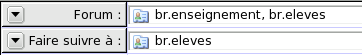
\includegraphics[width=0.45\textwidth]{images/cross_post_TB}
     & 
\includegraphics[width=0.45\textwidth]{images/cross_post_OE} \\
Thunderbird & Outlook Express
\end{tabular}
\vskip 12pt

C'est bien plus simple que d'envoyer successivement ton message sur tous les newsgroups, et la centralisation des r\'eponses permet de conserver un peu de clart\'e sur les newsgroups, tout en te facilitant la vie. Que des avantages donc!

\setcounter{page}{11}
